\documentclass{standalone}
\usepackage{tikz}
\usetikzlibrary{patterns, positioning}
\usepackage[sfdefault]{ClearSans} %% option 'sfdefault' activates Clear Sans as the default text font
\usepackage[T1]{fontenc}

\begin{document}
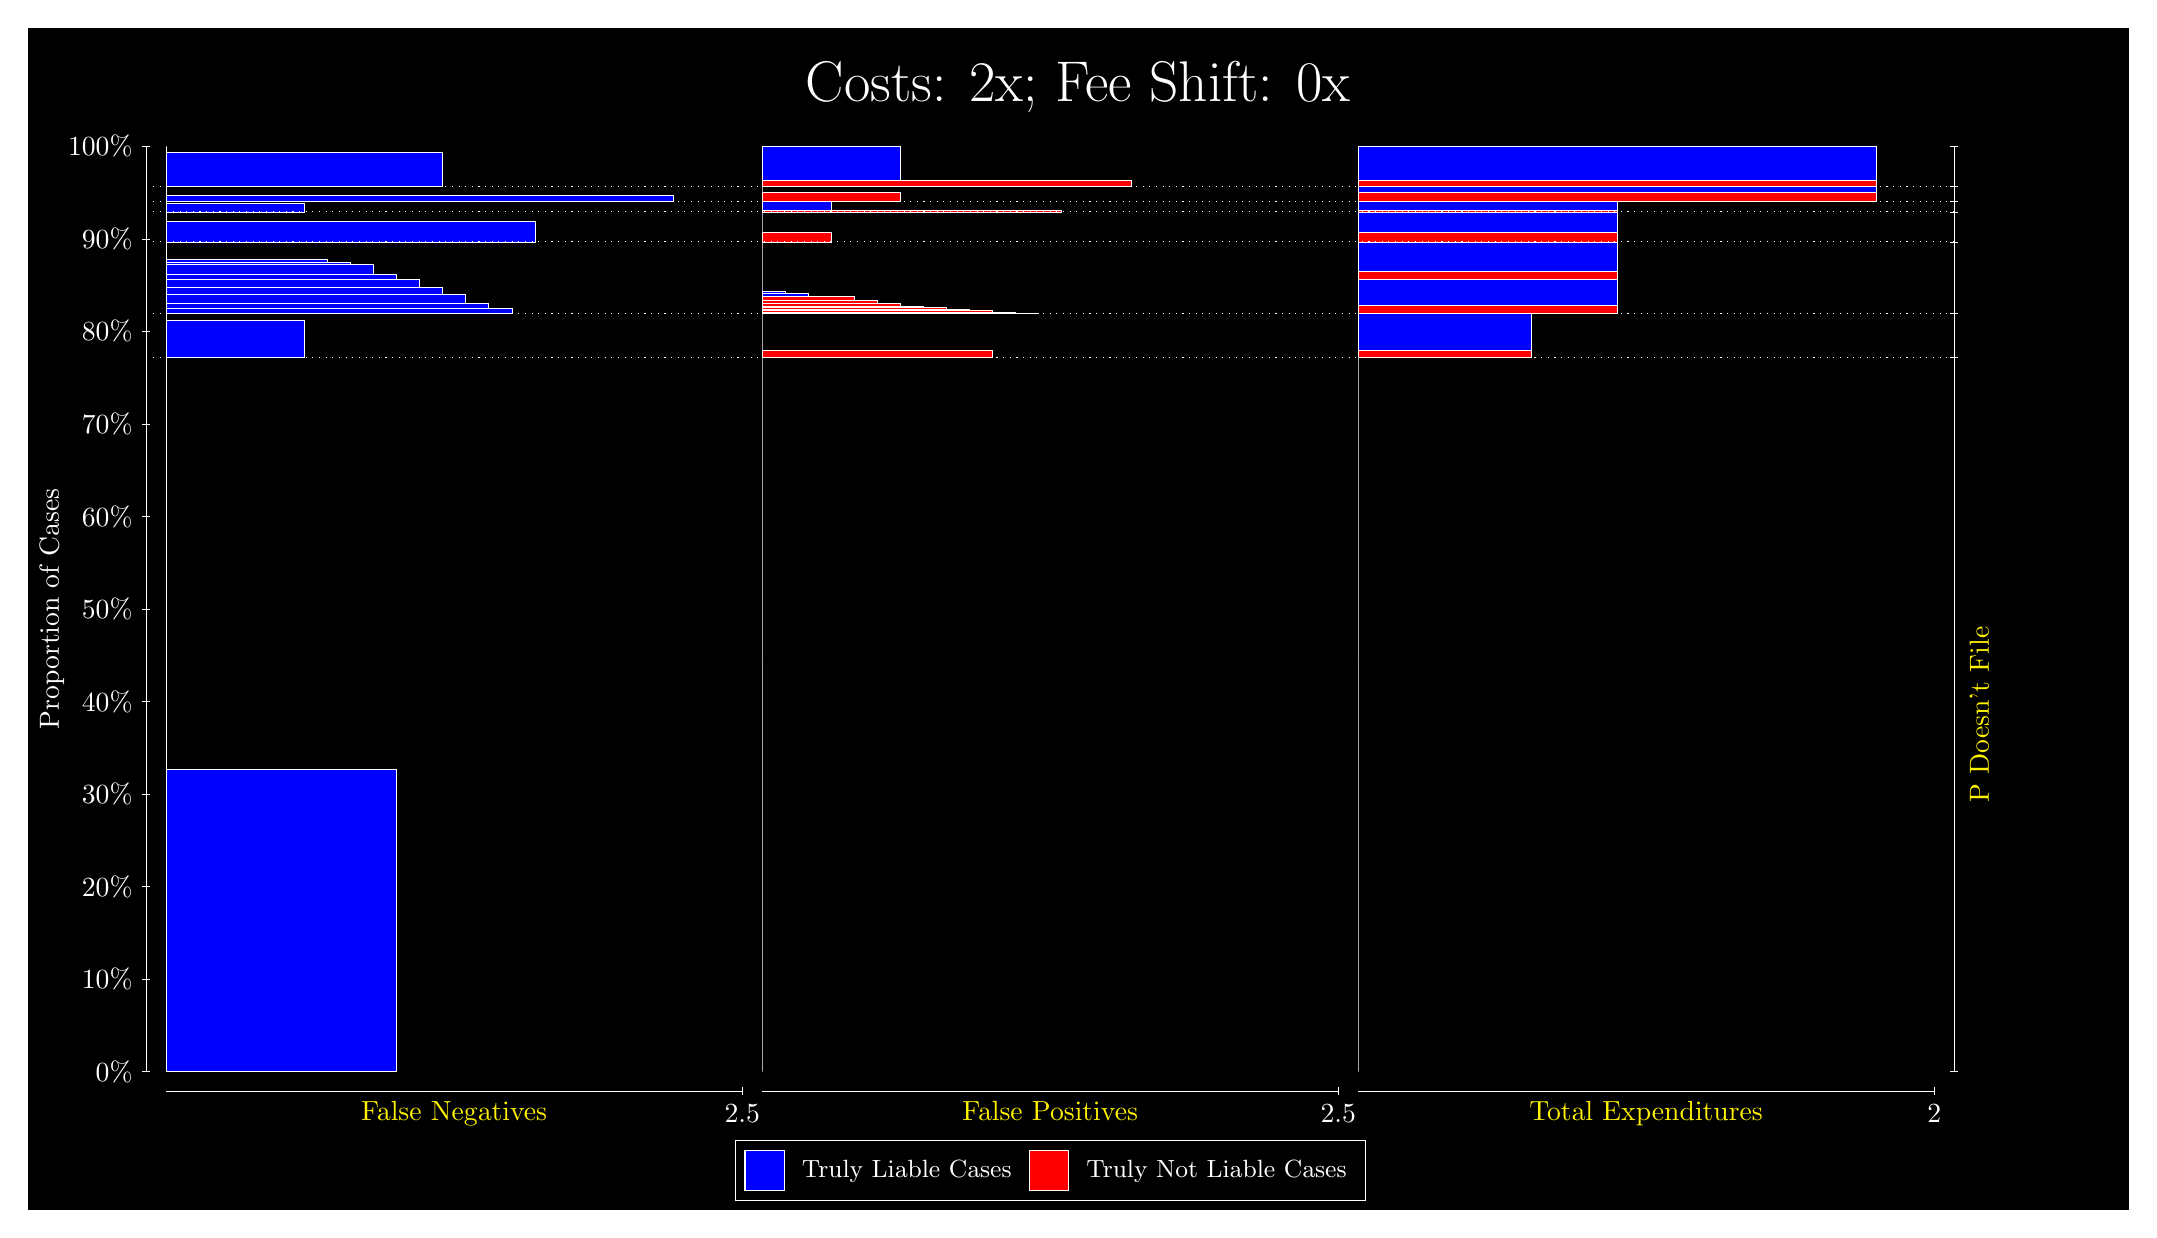
\begin{tikzpicture}
\draw[fill=black] (0,0) rectangle (26.667,15);
\draw[text=white] (0,13.5) rectangle (26.667,15) node[midway] {\huge Costs: 2x; Fee Shift: 0x};
\draw[white, very thin] (1.5,1.75) -- (1.5,13.5);
\node[rotate=90, text=white, anchor=center] at (0.3, 7.625) {Proportion of Cases};
\draw[white, very thin] (1.45,1.75) -- (1.55,1.75);
\node[text=white, anchor=east] at (1.45, 1.75) {0\%};
\draw[white, very thin] (1.45,2.925) -- (1.55,2.925);
\node[text=white, anchor=east] at (1.45, 2.925) {10\%};
\draw[white, very thin] (1.45,4.1) -- (1.55,4.1);
\node[text=white, anchor=east] at (1.45, 4.1) {20\%};
\draw[white, very thin] (1.45,5.275) -- (1.55,5.275);
\node[text=white, anchor=east] at (1.45, 5.275) {30\%};
\draw[white, very thin] (1.45,6.45) -- (1.55,6.45);
\node[text=white, anchor=east] at (1.45, 6.45) {40\%};
\draw[white, very thin] (1.45,7.625) -- (1.55,7.625);
\node[text=white, anchor=east] at (1.45, 7.625) {50\%};
\draw[white, very thin] (1.45,8.8) -- (1.55,8.8);
\node[text=white, anchor=east] at (1.45, 8.8) {60\%};
\draw[white, very thin] (1.45,9.975) -- (1.55,9.975);
\node[text=white, anchor=east] at (1.45, 9.975) {70\%};
\draw[white, very thin] (1.45,11.15) -- (1.55,11.15);
\node[text=white, anchor=east] at (1.45, 11.15) {80\%};
\draw[white, very thin] (1.45,12.325) -- (1.55,12.325);
\node[text=white, anchor=east] at (1.45, 12.325) {90\%};
\draw[white, very thin] (1.45,13.5) -- (1.55,13.5);
\node[text=white, anchor=east] at (1.45, 13.5) {100\%};

\draw[white, very thin] (24.457,1.75) -- (24.457,13.5);
\draw[white, very thin] (24.407,1.75) -- (24.507,1.75);
\node[anchor=west] at (24.407, 1.75) {};
\draw[white, very thin] (24.407,10.817) -- (24.507,10.817);
\node[anchor=west] at (24.407, 10.817) {};
\draw[white, very thin] (24.407,11.377) -- (24.507,11.377);
\node[anchor=west] at (24.407, 11.377) {};
\draw[white, very thin] (24.407,12.287) -- (24.507,12.287);
\node[anchor=west] at (24.407, 12.287) {};
\draw[white, very thin] (24.407,12.667) -- (24.507,12.667);
\node[anchor=west] at (24.407, 12.667) {};
\draw[white, very thin] (24.407,12.803) -- (24.507,12.803);
\node[anchor=west] at (24.407, 12.803) {};
\draw[white, very thin] (24.407,12.987) -- (24.507,12.987);
\node[anchor=west] at (24.407, 12.987) {};
\draw[white, very thin] (24.407,13.5) -- (24.507,13.5);
\node[anchor=west] at (24.407, 13.5) {};

\draw[white, very thin, fill=blue] (1.75,1.75) rectangle (4.6775,5.5868);
\draw[white, very thin, fill=red] (1.75,5.5868) rectangle (1.75,10.817);
\draw[white, very thin, fill=blue] (1.75,10.817) rectangle (3.5065,11.289);
\draw[white, very thin, fill=red] (1.75,11.289) rectangle (1.75,11.377);
\draw[white, very thin, fill=blue] (1.75,11.377) rectangle (6.1413,11.441);
\draw[white, very thin, fill=blue] (1.75,11.441) rectangle (5.8486,11.512);
\draw[white, very thin, fill=blue] (1.75,11.512) rectangle (5.5558,11.617);
\draw[white, very thin, fill=blue] (1.75,11.617) rectangle (5.2631,11.706);
\draw[white, very thin, fill=blue] (1.75,11.706) rectangle (4.9703,11.811);
\draw[white, very thin, fill=blue] (1.75,11.811) rectangle (4.6775,11.88);
\draw[white, very thin, fill=blue] (1.75,11.88) rectangle (4.3848,11.999);
\draw[white, very thin, fill=blue] (1.75,11.999) rectangle (4.092,12.033);
\draw[white, very thin, fill=blue] (1.75,12.033) rectangle (3.7993,12.067);
\draw[white, very thin, fill=red] (1.75,12.067) rectangle (1.75,12.287);
\draw[white, very thin, fill=blue] (1.75,12.287) rectangle (6.4341,12.542);
\draw[white, very thin, fill=red] (1.75,12.542) rectangle (1.75,12.667);
\draw[white, very thin, fill=blue] (1.75,12.667) rectangle (3.5065,12.776);
\draw[white, very thin, fill=red] (1.75,12.776) rectangle (1.75,12.803);
\draw[white, very thin, fill=blue] (1.75,12.803) rectangle (8.1906,12.878);
\draw[white, very thin, fill=red] (1.75,12.878) rectangle (1.75,12.987);
\draw[white, very thin, fill=blue] (1.75,12.987) rectangle (5.2631,13.423);
\draw[white, very thin, fill=red] (1.75,13.423) rectangle (1.75,13.5);
\draw[white, very thin, fill=red] (9.3189,1.75) rectangle (9.3189,6.9798);
\draw[white, very thin, fill=blue] (9.3189,6.9798) rectangle (9.3189,10.817);
\draw[white, very thin, fill=red] (9.3189,10.817) rectangle (12.246,10.905);
\draw[white, very thin, fill=blue] (9.3189,10.905) rectangle (9.3189,11.377);
\draw[white, very thin, fill=red] (9.3189,11.377) rectangle (12.832,11.383);
\draw[white, very thin, fill=red] (9.3189,11.383) rectangle (12.539,11.39);
\draw[white, very thin, fill=red] (9.3189,11.39) rectangle (12.246,11.412);
\draw[white, very thin, fill=red] (9.3189,11.412) rectangle (11.954,11.428);
\draw[white, very thin, fill=red] (9.3189,11.428) rectangle (11.661,11.453);
\draw[white, very thin, fill=red] (9.3189,11.453) rectangle (11.368,11.474);
\draw[white, very thin, fill=red] (9.3189,11.474) rectangle (11.075,11.513);
\draw[white, very thin, fill=red] (9.3189,11.513) rectangle (10.783,11.544);
\draw[white, very thin, fill=red] (9.3189,11.544) rectangle (10.49,11.597);
\draw[white, very thin, fill=blue] (9.3189,11.597) rectangle (9.9044,11.631);
\draw[white, very thin, fill=blue] (9.3189,11.631) rectangle (9.6116,11.665);
\draw[white, very thin, fill=blue] (9.3189,11.665) rectangle (9.3189,12.287);
\draw[white, very thin, fill=red] (9.3189,12.287) rectangle (10.197,12.412);
\draw[white, very thin, fill=blue] (9.3189,12.412) rectangle (9.3189,12.667);
\draw[white, very thin, fill=red] (9.3189,12.667) rectangle (13.125,12.693);
\draw[white, very thin, fill=blue] (9.3189,12.693) rectangle (10.197,12.803);
\draw[white, very thin, fill=red] (9.3189,12.803) rectangle (11.075,12.911);
\draw[white, very thin, fill=blue] (9.3189,12.911) rectangle (9.3189,12.987);
\draw[white, very thin, fill=red] (9.3189,12.987) rectangle (14.003,13.064);
\draw[white, very thin, fill=blue] (9.3189,13.064) rectangle (11.075,13.5);
\draw[white, very thin, fill=red] (16.888,1.75) rectangle (16.888,6.9798);
\draw[white, very thin, fill=blue] (16.888,6.9798) rectangle (16.888,10.817);
\draw[white, very thin, fill=red] (16.888,10.817) rectangle (19.083,10.905);
\draw[white, very thin, fill=blue] (16.888,10.905) rectangle (19.083,11.377);
\draw[white, very thin, fill=red] (16.888,11.377) rectangle (20.181,11.485);
\draw[white, very thin, fill=blue] (16.888,11.485) rectangle (20.181,11.806);
\draw[white, very thin, fill=red] (16.888,11.806) rectangle (20.181,11.919);
\draw[white, very thin, fill=blue] (16.888,11.919) rectangle (20.181,12.287);
\draw[white, very thin, fill=red] (16.888,12.287) rectangle (20.181,12.412);
\draw[white, very thin, fill=blue] (16.888,12.412) rectangle (20.181,12.667);
\draw[white, very thin, fill=red] (16.888,12.667) rectangle (20.181,12.693);
\draw[white, very thin, fill=blue] (16.888,12.693) rectangle (20.181,12.803);
\draw[white, very thin, fill=red] (16.888,12.803) rectangle (23.475,12.911);
\draw[white, very thin, fill=blue] (16.888,12.911) rectangle (23.475,12.987);
\draw[white, very thin, fill=red] (16.888,12.987) rectangle (23.475,13.064);
\draw[white, very thin, fill=blue] (16.888,13.064) rectangle (23.475,13.5);
\draw[white, dotted] (1.5,10.817) -- (24.457,10.817);
\draw[white, dotted] (1.5,11.377) -- (24.457,11.377);
\draw[white, dotted] (1.5,12.287) -- (24.457,12.287);
\draw[white, dotted] (1.5,12.667) -- (24.457,12.667);
\draw[white, dotted] (1.5,12.803) -- (24.457,12.803);
\draw[white, dotted] (1.5,12.987) -- (24.457,12.987);
\draw[white, very thin] (1.75,1.5) -- (9.0689,1.5);
\node[text=yellow, anchor=north] at (5.4094, 1.5) {False Negatives};
\draw[white, very thin] (9.0689,1.45) -- (9.0689,1.55);
\node[text=white, anchor=north] at (9.0689, 1.45) {2.5};

\draw[white, very thin] (9.3189,1.5) -- (16.638,1.5);
\node[text=yellow, anchor=north] at (12.978, 1.5) {False Positives};
\draw[white, very thin] (16.638,1.45) -- (16.638,1.55);
\node[text=white, anchor=north] at (16.638, 1.45) {2.5};

\draw[white, very thin] (16.888,1.5) -- (24.207,1.5);
\node[text=yellow, anchor=north] at (20.547, 1.5) {Total Expenditures};
\draw[white, very thin] (24.207,1.45) -- (24.207,1.55);
\node[text=white, anchor=north] at (24.207, 1.45) {2};

\node[text=yellow, centered, rotate=90] at (24.777, 6.2833) {P Doesn't File};







\draw (12.978300999999998,1.5) node[draw=none] (baseCoordinate) {};
\begin{scope}[align=center]
        \matrix[scale=0.5, draw=white, below=0.5cm of baseCoordinate, nodes={draw}, column sep=0.1cm]{
            \node[rectangle, draw, minimum width=0.5cm, minimum height=0.5cm, fill=blue] {}; &
            \node[draw=none, font=\small, text=white] (B) {Truly Liable Cases}; &
            \node[rectangle, draw, minimum width=0.5cm, minimum height=0.5cm, fill=red] {}; &
            \node[draw=none, font=\small, text=white] (B) {Truly Not Liable Cases}; \\
            };
\end{scope}

\end{tikzpicture}
\end{document}